\documentclass[11pt, a4paper]{article}
\usepackage[a4paper, margin=1in]{geometry}
\usepackage[english]{babel}
\usepackage{blindtext}
\usepackage{amsmath}
\usepackage{amssymb}
\usepackage{epsfig}
\usepackage{graphicx}
\usepackage{float}

\begin{document}

\begin{titlepage}
  \centering
  \title{ROTA \\\large Remotely Operated Transportation Apperatus \\\small \textbf{Rijksuniversiteit Groningen}}
  \author{Sebastiaan van Houttum - S3146391 \\ Oliver Strik - S3100693}
  \date{November 2017}
  \maketitle
  \thispagestyle{empty}
  %\includegraphics[width=0.5\textwidth]{images\RUGLOGO.eps}\\[0.5cm]
\end{titlepage}

\pagebreak\tableofcontents\pagebreak
% Sections
\section{Problem Description}
\par
We always had the idea to make something ridiculous, such as a toy car that drives around by controlling it from your phone. The device would need wifi, a way of receiving and processing input, and a way to give information about its surroundings.

\section{Problem Analysis}
\par
In order to get the project off the ground, we started with making a plan. Our plan would consist of two parts, designing the code and the hardware

Can we make a toy car drive around, avoiding obstacles automatically?

Given the fact that our current project is relatively small, and the limited amount of time that we have for this, we concluded it best to simplify our problem as follows:

Can we mod or hack an RC car such that we can control it over wifi?



%===evaluation===
This would allow us a proof of concept which could be expanded when we have any remaining time. If time remained, we could add the following features:

 - Obstacle detection
 - Camera feedback
 - Different body
 - Accelerometer to check if we've actually hit something


\section{Design}
\par
In order to build the car, the following hardware was used:
\begin{itemize}
\item Arduino Uno
\item Velleman Stepper Motor Controller
\item Servo from the Arduino started kit
\item Raspberry Pi B Model (v1.2)
\item Generic WiFi USB Adapter
\item 8GB Micro SD card
\item RC car which would have otherwise been forgotten about
\item Power bank with 2 USB ports to power the Arduino
\item Jumper wires
\item 9V block
\end{itemize}
The Raspberry Pi was first configured by loading the Raspbian OS on it, but this proved to be flawed when setting up a WiFi network on the Pi, since there were many complications with the network. Therefore, it was decided Arch Linux would be better suited. A server for the Raspberry Pi with which our app communicates was then written in C.

The server and app were designed such that the app sends a packet describing the position of the two joysticks, this packet consists of a total of 5 bytes. Two for each joystick and an extra one in case something needed to be added at a later date. The server receives this packet from the app, and sends it via a serial connection to the Arduino. This is then read by the Arduino, which translates the packet into the motor speed and servo direction.

At the same time, the controller app was developed. Android was decided as deployment platform, because of its expansive support documentation and general ease of use. The app would have two joysticks, and sends a packet of 5 bytes to our server. The packet contains an undefined byte, the x and y for the left joystick and the x and y for the right.

The last piece to develop was the code for the Arduino to interpret the packet of data sent to it from the server.

Finally, it was just a matter of assembling the components. After piling all the components listed above on to an old RC car frame, the result was an odd looking Android controlled RC Car.

\section{Program Code}
\par The code of ROTA is split into three seperate programs.
\begin{itemize}
  \item The controller - Written in Java. https://github.com/Kranex/ROTA-Controller
  \item The Server - Written in C. https://github.com/Kranex/ROTA-Server
  \item The Interpreter - Written in Arduino C/C++. https://github.com/NotSoScientific/ROTA-Interpreter
\end{itemize}
In the interest of saving trees, the 700+ lines of code are not included in this document,
if you wish to find them please use the links above to access them. A description of
each program, however, is provided below.

\subsection{The Controller}
\par
The controller was written in Java with the help of the Android Studio IDE.
The main function of the controller is to create two floating joysticks to allow
users to submit input to ROTA. It is essentially an Xbox or PlayStation controller
but without any buttons.
One joystick is created on the left and one on the right, they will place themselves
under the first touch on their half of the screen and the centre of the joystick
will remain at that point until the finger is lifted again. This allows for some degree of personal adjustability; not everyone holds their phone the same way,
and not all phones are the same size or shape, so the joysticks should not be fixed
to one place on the screen.

\par
The controller also tries to connect to a TCP socket on the IP address 192.168.12.1
port 55455, the Raspberry Pi was set up to maintain a consistent gateway address
so that the controller would never have to ask for the IP address of the server,
the server was also configured to only use port 55455.
Once a connection has been created the controller will send an update packet every
few miliseconds. This packet consists of 5 bytes \{a,x1,y1,x2,y2\}.
\begin{enumerate}
  \item 'a' is an undefined byte. It can be used for anything; it was added in case
   some kind of status update or emergency stop button was introduced.
  \item x1 and y1 are the influences of the left joystick. Their value will be
  between -127 to 127. (0,0) would mean the joystick is centered. (0,127) would mean
  the joystick was centered on the x-axis but pushed all the way up on the y-axis.
  \item x2 and y2 are just the same as x1 and y1 but are for the right joystick.
\end{enumerate}
The packet does not require any leading or ending byte as TCP guarantees that all
packets will arrive and they will all arrive in the correct order. Thus, on the server,
if the Server reads 5 bytes it will always read \{a,x1,y1,x2,y2\} if a packet exists to be read.

\subsection{The Server}
\par The server is by far the most convoluted program of the three, which is thanks
to it having been programmed in C.
It does only one thing:
 forward all packets received from the controller, straight to the Arduino over serial.
It does, however, add 127 to each of the signed bytes as the serial connection
seemed to really dislike the signed bytes. 127 is then immediately subtracted from
the byte when it gets to the Arduino.
This is all handled in about 5 lines of code, however, there are nearly 300 lines
surrounding it most of which is simply initialisation for the TCP server and serial
connection.
On the Raspberry Pi, the server is added to the list of programs to start at boot
with systemd, thus no login is required, the Raspberry Pi must only be booted for
the server to be created.

\subsection{The Interpreter}
\par The interpreter, for lack of a better name, is the program running on the Arduino
which `interprets' the x and y influences recieved from the server and translates them
into motor speed, servo angle or whatever else we happen to connect to ROTA.
This job could have been done with the Raspberry Pi alone, however, we would then have
had the constraints of few GPIO to communicate with, as well as the lower voltage of
the GPIO (3.3V instead of 5V) to deal with. Thus we decided to use the Arduino as the
step between the Raspberry Pi and the extra peripherals.
\par After initialising the serial connections and any global variables, the arduino then
reads a single byte from the serial buffer and acts upon it. It keeps count of which particular
byte it is reading and then, as we have it currently set up, if it is the left y, uses
it to set the motor speed and direction or if it is the right x, use it to set the
servo angle. The particular stick or axis that controls each of these can easily be changed,
the only reason we have it set up as so is that it made practical sense to split
the controls of throttle and steering on to separate sticks. As for why the sticks
are capable of moving in both axis when only one is required, it doesn't impair their
function, it was easier to make two identical joysticks over two unique ones and
most importantly, if we had the time and the servos to do it, we would have like to
have added a moveable camera. Unfortunately, this was not the case, but now at least
it features the ability to have such a camera with the addition of only two if statements.

\section{Tests and Results}
\par
\begin{figure}[H]
\centering
  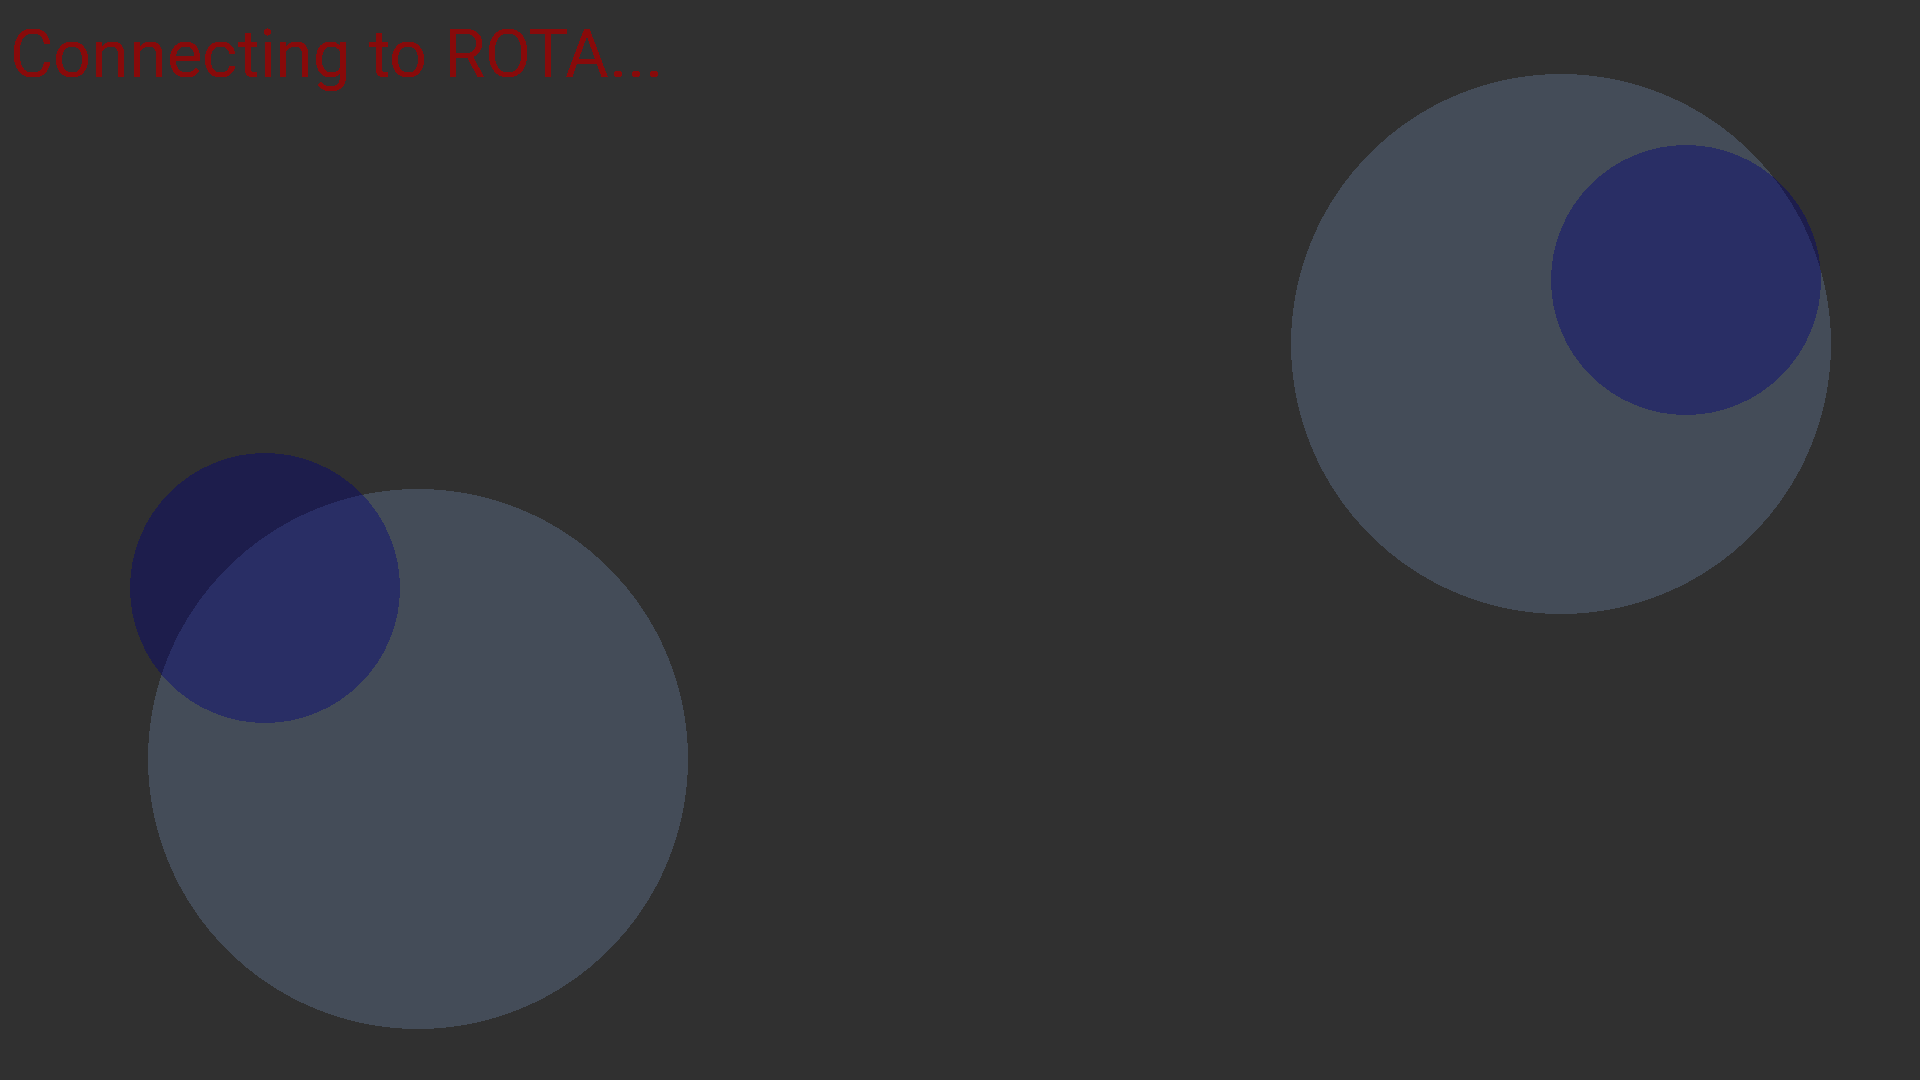
\includegraphics[width=0.6\textwidth]{sections/testRes/app1}
    \caption{A photo showing the joysticks in the app.}
\end{figure}
\begin{figure}[H]
\centering
  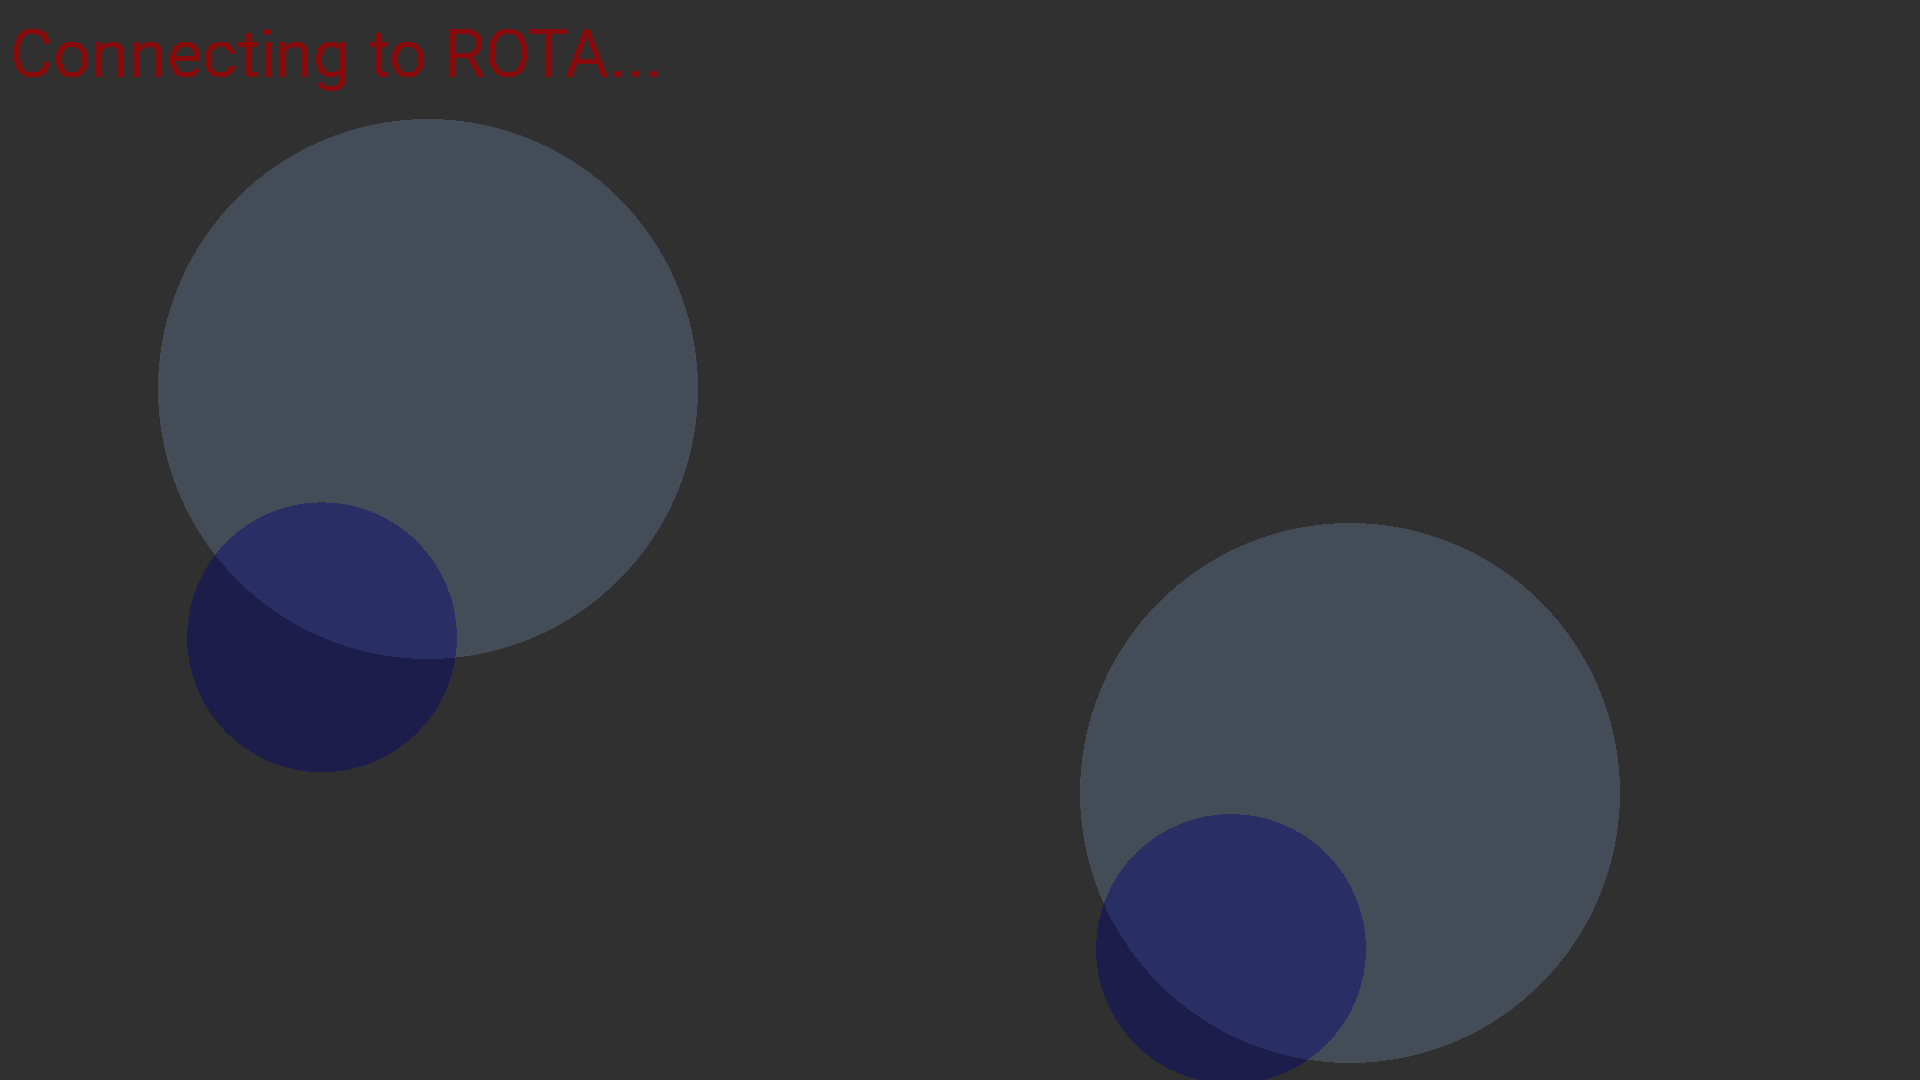
\includegraphics[width=0.6\textwidth]{sections/testRes/app2}
    \caption{Another photo showing the joysticks in the app. This shows how the joysticks will move when the user touches the screen.}
\end{figure}
\begin{figure}[H]
\centering
  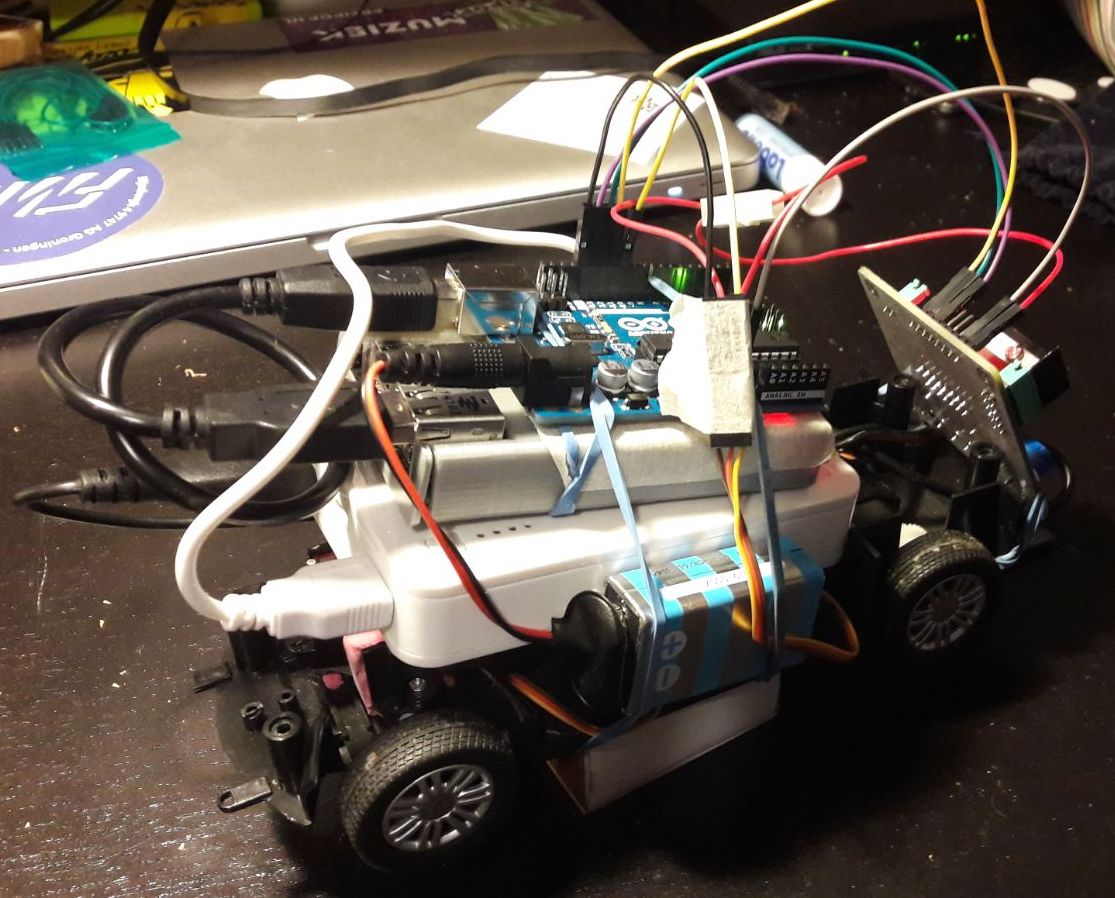
\includegraphics[width=0.6\textwidth]{sections/testRes/left}
    \caption{A view of the left side of the finished car.}
\end{figure}
\begin{figure}[H]
\centering
  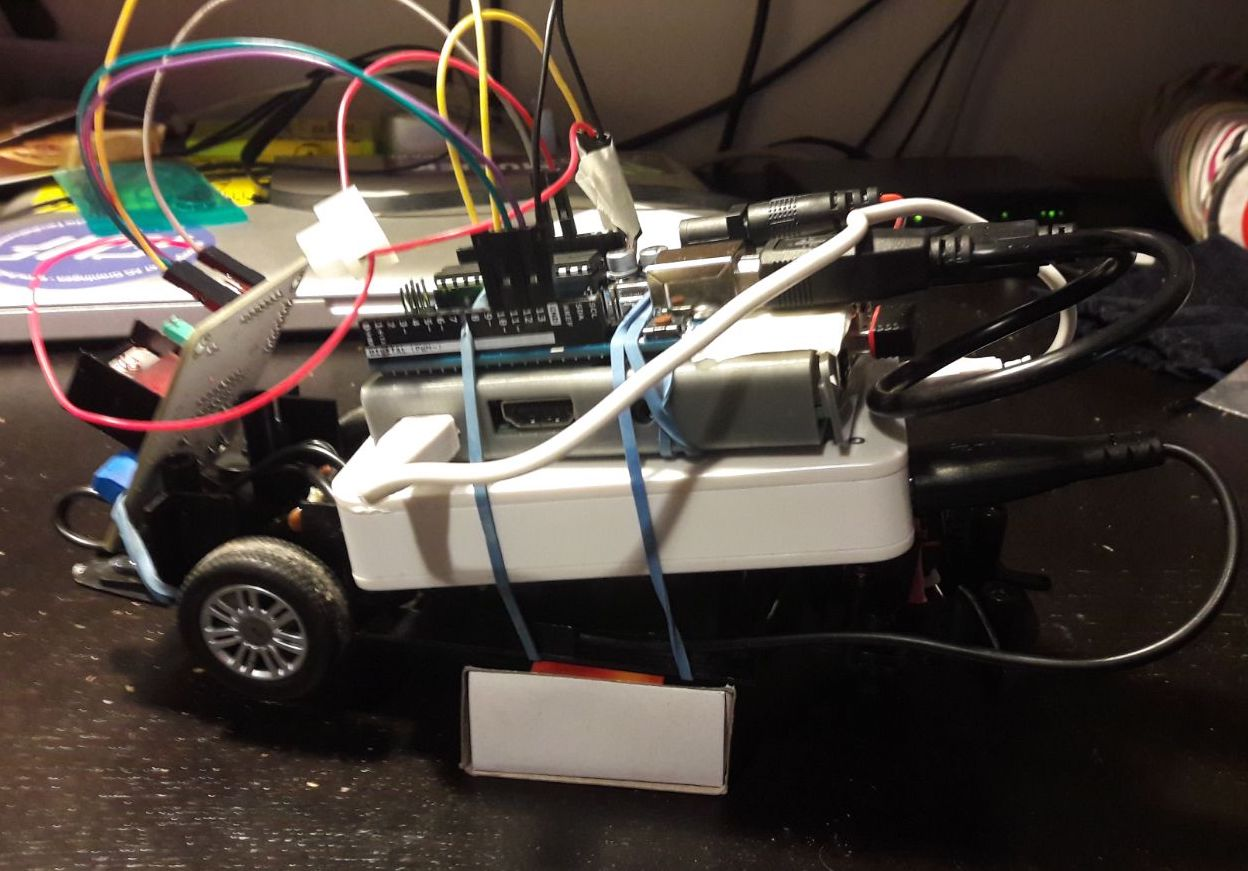
\includegraphics[width=0.6\textwidth]{sections/testRes/right}
    \caption{A view of the right side of the finished car. You may notice the missing front wheel that was being repaired at the time of this photograph.}
\end{figure}
\begin{figure}[H]
\centering
  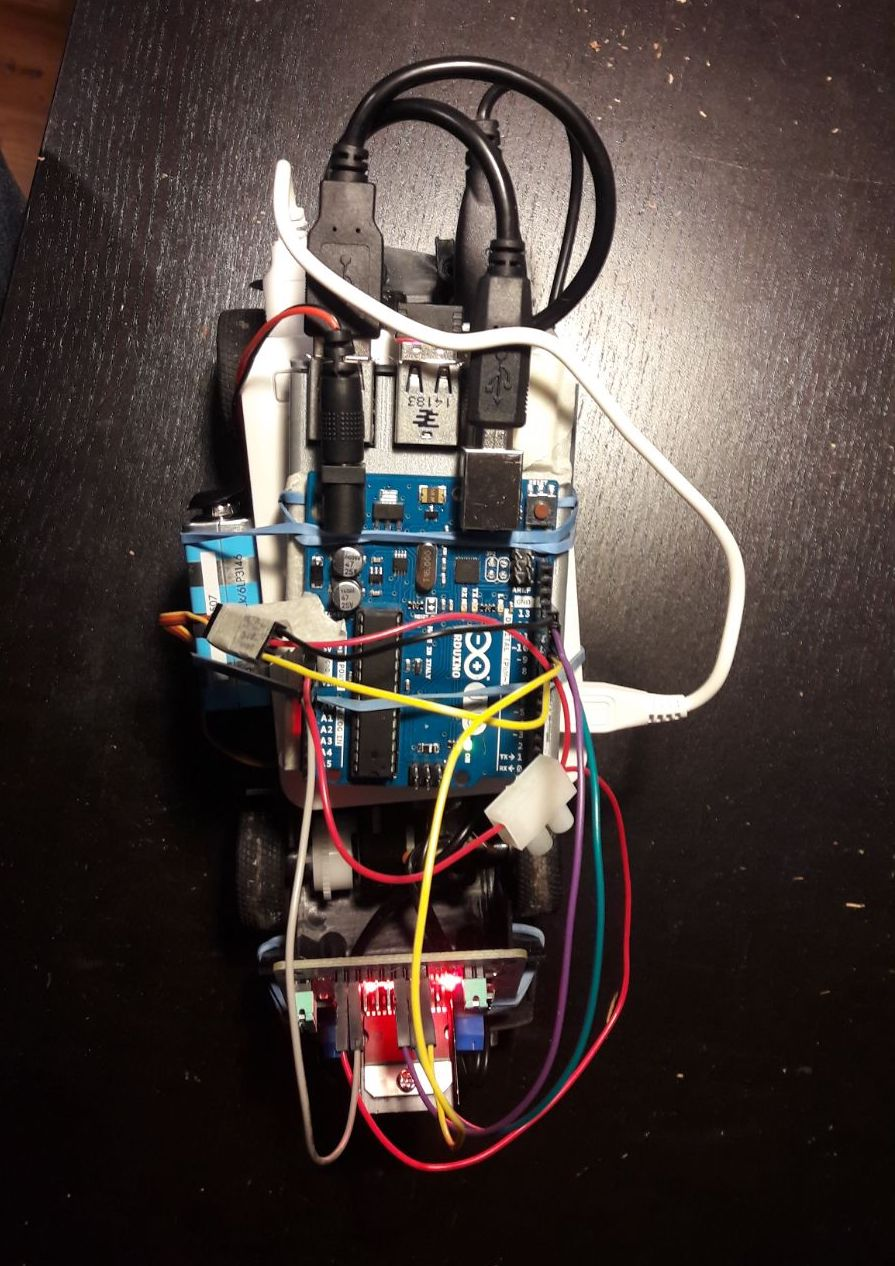
\includegraphics[width=0.6\textwidth]{sections/testRes/top}
    \caption{A view of the top of the finished car.}
\end{figure}

\section{Evaluation}
\par Throughout the development of ROTA there have been things that needed to be tested.
After all, there are three devices that could fail. The first thing that was programmed was
the app, after fixing many small issues that showed up throughout development, three major
problems showed.  
\begin{enumerate}
  \item If the app is disconnected from the server, by losing the wifi or something
  similar, it would never reconnect. To fix this, the client initialisation thread was
  extended to perpetually loop, if the client was not connected, it would try to reconnect it,
  otherwise, it would send an update packet. This also helped limit the number of packets
  being sent to the server as originally a packet would be sent every time the user
  stimulated the touch screen, this helped prevent the Arduino from becomming overloaded.
  \item If the screen focus shifts, causing the app to leave fullscreen, it never reverts.
  This does not impact usability, however it is annoying. This was fixed by giving the
  Android immersive environment the sticky flag. Now, popups and dragging the system bar into
  view does not resize the app as they are rendered 'over' the app. When they disappear
  the app is still fullscreen.
  \item If the user leaves the app, Android will `suspend' it. This is great, however,
  it wreaks havoc with the server connection. Very strange things can happen, the best
  you can hope for is that the app crashes, at worst, the app tries to reistablish the
  connection and you end up with 5 or 6 rogue threads spamming TCP Requests.
  To prevent this, the app was set up to destroy itself completely when minimised. This
  loses no functionality, however, as the app would have to be restarted when it comes
  out of suspension anyway, it is just easier to restart from the beginning of the program.
\end{enumerate}
There were never really any issues with the server, par some minor confusion caused by
C's lack of a 'byte' type and chars being unsigned on some systems but not others.
This was easily fixed by declaring all chars, being used as bytes, as signed chars.
\par
Another problem came with the Arduino, it would not accept signed bytes across serial.
this meant that either the transmission method needed to be revised or that unsigned bytes
needed to be sent instead. As all bytes were between -127 and 127, adding 127 before sending
and subtracting it after receiving solved this problem.
\par
The biggest problem of them all was how to supply power to the Arduino,
the Raspberry Pi, and the motor shield. In the end, it was decided the Raspberry Pi and
the motor shield would receive power from a large USB power bank. The Raspberry Pi would
then power the Arduino. This seemed to work on the bench when the Arduino was plugged into
the PC for tuning the servo and running light tests on the motor. However, the Raspberry Pi
could not deliver the current to the Arduino to power the servo and the logic side of the
motor controller, this would crash the Raspberry Pi and all hell would break loose.
To counter this issue the Arduino was given its very own 9v battery. While this is not
perfect, it does seem to solve the problem. Ideally a dedicated Lithium Polymer
battery would have been preferred, a 2200mah 7.4v LiPo would be small and light enough
to fit on the frame, however, they are not exactly cheap and the Raspberry Pi would require
something extra to step the voltage down to 5v.
\par
After the power problem was sorted, the car worked almost perfectly, it can pick up quite
some speed, every now and then there is a slight delay in the controls however not enough
to cause serious issues. The exact reason for the delay is not understood, amongst other things
it could be due to the Arduino being flooded with more packets than it can handle, or it
could be because the Raspberry Pi suffers from a similar problem. The only minor faults are
that the servo is rather poorly attached to the steering, allowing for a small margin of
free movement. This means that the steering is never exactly centered and the car needs
constant steering adjustments to stay on course. It was also noticed that the front wheels
would lock on the frame when turning. This was because all the weight had crushed the suspension.
To fix this the wheel arches were removed.


\begin{thebibliography}{3}
\bibitem{Controller}
Strik, O.H.P (2017). The Source Code for the ROTA Android Controller. Available on: https://www.github.com/Kranex/ROTA-Controller
\bibitem{Server}
Strik, O.H.P (2017). The Source Code for the ROTA Server. Available on: https://www.github.com/Kranex/ROTA-Server
\bibitem{Interpreter}
Houttum, S.F.W.M van (2017). The Source Code for the Arduino interpreter program. Available on: https://www.github.com/NotSoScientific/ROTA-Interpreter
\end{thebibliography}

%\pagebreak\input{references}
%\pagebreak\input{appendix}
\end{document}
